%   %==========================================================================
%   %  Section
%   %==========================================================================
    \section{ビオ$=$サバールの法則(復習)}
        \begin{mycomment}
            ビオ$=$サバールの法則についての詳細は,\ref{subsec:BiotSavart_Gene}節を参照.
            以下は,そこからの抜粋である.
        \end{mycomment}

        ビオ$=$サバールの法則は,磁束密度に関する法則である.
        \begin{myshadebox}{ビオ$=$サバールの法則(電流密度表示)}
            電流はその周囲に磁束密度を発生させる.その発生は以下の式に従う.
            \begin{align}
                \bB(\br)
                = \frac{\mu_{0}}{4\pi}
                    \int \frac{ \bi(\br')\times (\br-\br') }{ |\br-\br'|^{3} } \df V'.
            \end{align}
        \end{myshadebox}
        \begin{figure}[hbt]
            \begin{center}
                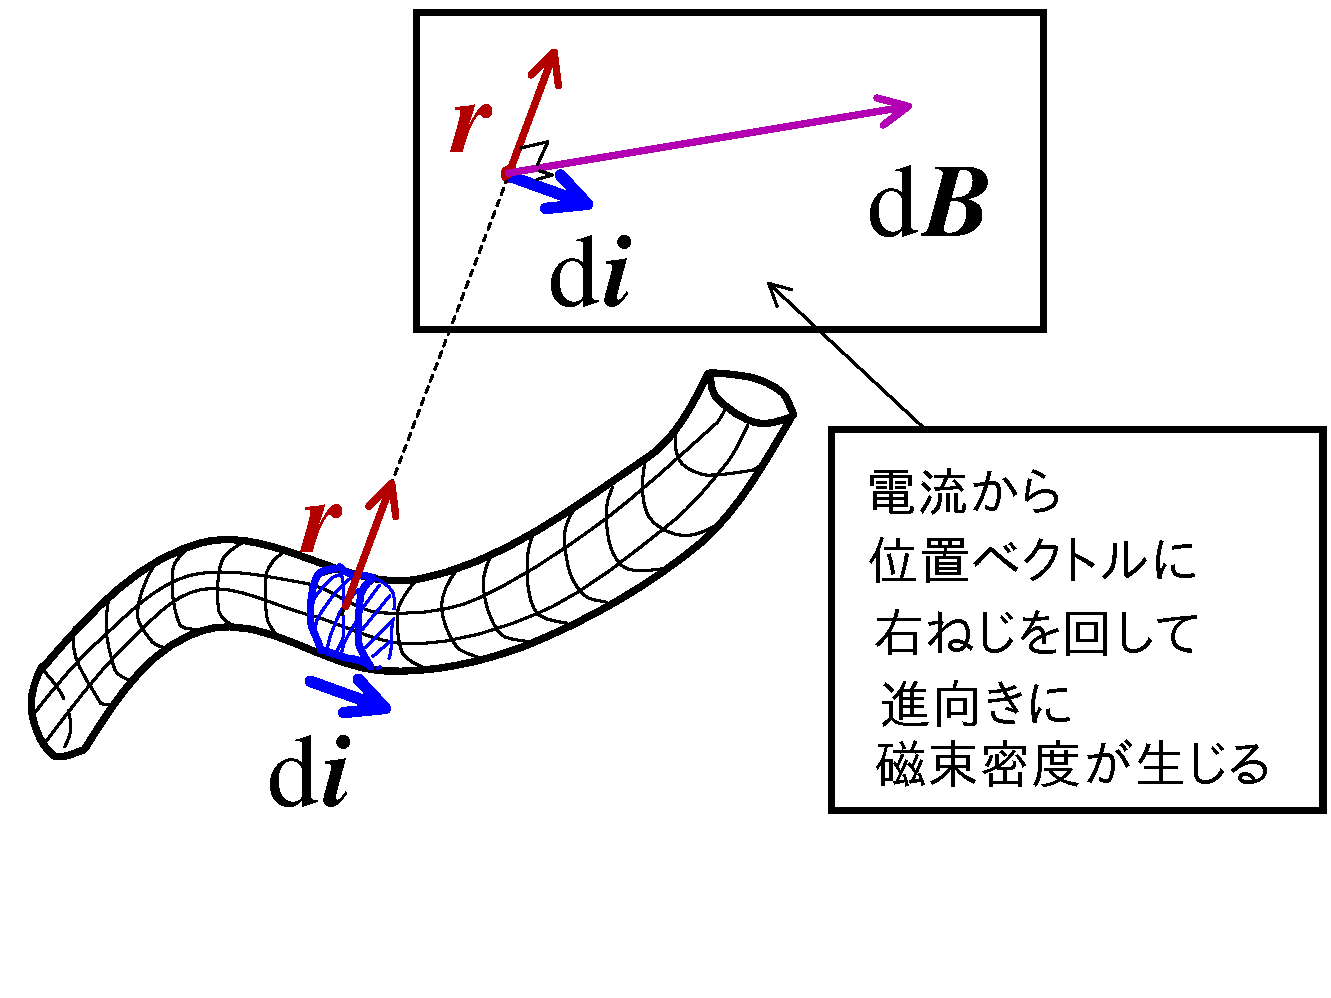
\includegraphics[keepaspectratio, width=7.2cm, height=5.79cm, clip]{biot_savart_1.pdf}
                \caption{ビオ$=$サバールの法則}
            \end{center}
        \end{figure}


%   %==========================================================================
%   %  Section
%   %==========================================================================
    \section{磁束密度に対するガウスの法則の導出}
%   %==========================================================================
%   %  Subsection
%   %==========================================================================
    \subsection{公式の確認}
        ビオ$=$サバールの法則から,磁束密度に対するガウスの法則を導出する
        手順を示す.まず,導出の際に以下のベクトル解析の公式を使用する.
            \begin{align}\label{eq:kousiki_kakunin}
                \dgrad \left( \frac{1}{r} \right) = - \frac{\br}{r^{3}}.  \\
                \drot (a\bX) = (\dgrad a) \times \bX + a(\drot \bX).
            \end{align}
        ただし,$r=\sqrt{x^{2}+y^{2}+z^{2}}$ である.また,$a$ は任意の
        スカラー関数であり,$\bX$ はベクトル関数である.

        \begin{memo}{公式の変形1}
            この公式を使うのだけど,このまま適用するわけではない.
            適用しやすいように,形を変えておこう.上段の式から見ていこう.
                \begin{equation*}
                    \dgrad \left( \frac{1}{r} \right) = - \frac{\br}{r^{3}}.
                \end{equation*}
            の $\br$ に注目する.任意の定ベクトル $\bC$ を考えて,$\br$ を
                \begin{equation*}
                    \br \rightarrow \br - \bC
                \end{equation*}
            と置き換えてやる.すると
                \begin{equation*}
                    \dgrad \left( \frac{1}{|\br - \bC|} \right)
                    =
                    - \frac{\br - \bC}{{|\br - \bC|}^{2}}
                \end{equation*}
            となる
        \footnote{
                    計算は合成微分を繰り返し.面倒だが,$x$ 成分の
                    計算だけでよいので,手で計算してほしい.
                    ここでは,記述が面倒なので,結果のみとする.
                }.
        \end{memo}

        \begin{memo}{公式の変形2}
            任意の定ベクトル $\bX$ に対して,
                \begin{equation*}
                    \drot \bX = \b0
                \end{equation*}
            が成立するとき,
                \begin{equation*}
                    \drot (a\bX) = (\dgrad a) \times \bX
                \end{equation*}
            が成り立つ.
        \end{memo}

%   %==========================================================================
%   %  Subsection
%   %==========================================================================
    \subsection{導出}
        ベクトル解析の公式 $\ddiv (\drot \bX) = 0$ を念頭に置き,
        ビオ$=$サバールの法則の式を変形していこう.

        まず,ビオ$=$サバールの式を書き下す.
            \begin{align}
                \bB(\br)
                =\frac{\mu_{0}}{4\pi}
                \int\frac{\bi(\br')\times
                (\br-\br')
                }{|\br-\br'|^{3}}\df V'.
            \end{align}
        この式の
            \begin{equation*}
                \frac{\br-\br'}{|\br-\br'|^{3}}
            \end{equation*}
        の部分の注目すると,公式
            \begin{equation*}
                \dgrad \left( \frac{1}{|\br - \bC|} \right)
                =
                - \frac{\br - \bC}{{|\br - \bC|}^{2}}
            \end{equation*}
        から
            \begin{align}
                \bB(\br)
                =\frac{\mu_{0}}{4\pi}
                    \int
                        \bi(\br')\times
                            \biggl\{
                                - \dgrad \left( \frac{1}{|\br - \br'} \right)
                            \biggr\}
                    \df V'.
            \end{align}
        さらに,公式($\bU$ は定ベクトル,$a$ はスカラー関数)
            \begin{align*}
                \drot (a\bU) &= (\dgrad a) \times \bU  \\
                             &= -\bU \times (\dgrad a)  \\
                             &= \bU \times (- \dgrad a)
            \end{align*}
        により,
            \begin{align*}
                \bB(\br)
                &=\frac{\mu_{0}}{4\pi}
                    \int
                        \bi(\br')\times
                            \biggl\{
                                - \dgrad \left( \frac{1}{|\br - \br'|} \right)
                            \biggr\}
                    \df V'
                 \\
                &= \int
                        \drot \left( \bi(\br') \frac{1}{|\br - \br'|} \right)
                    \df V'
                 \\
                &= \int
                        \drot \left(\frac{ \bi(\br') }{|\br - \br'|} \right)
                    \df V'.
            \end{align*}
        積分と微分の順番を変更して,
            \begin{align}
                \bB = \drot \int \left(\frac{ \bi(\br') }{|\br - \br'|} \right) \df V'.
            \end{align}

        ここで,次のようなベクトル関数を定義する.
            \begin{align}
                \bA(\br) := \int \frac{ \bi(\br') }{|\br - \br'|} \df V'.
            \end{align}
        これは後で \textbf{ベクトル$\cdot$ポテンシャル} と呼ばれる量と同じものである
            \footnote{
                ここでは,あくまでも形式的に導入するものであり,その正式な導入は後で行う.
            }.
        この $\bA(\br)$ をにより,ビオ$=$サバールの法則は以下のような形になる.
            \begin{align}
                \bB(\br) = \drot \bA(\br).
            \end{align}

        ここまで計算すれば,明らかだ.両辺に $\ddiv$ をとろう.
            \begin{align}
                \ddiv \bB(\br) &= \ddiv \left( \drot \bA(\br) \right). \notag \\
                \therefore \quad
                \ddiv \bB(\br) = 0.
            \end{align}
        この計算で,公式 $\ddiv (\drot \bX) = 0$ を使った.
        これは,磁束密度に対するガウスの法則に他ならない.

        以上の計算から,ビオ$=$サバールの法則に従って生じる磁束密度は,
        ガウスの法則 $\ddiv \bB(\br) = 0$ を満たすことが示された.


%   %==========================================================================
%   %  Subsection
%   %==========================================================================
    \subsection{まとめ}
        以上の結果をまとめよう.
                    \begin{myshadebox}{静磁束密度のガウスの法則(微分形)}
                        時間変化のない磁束密度に対する,局所的な
                        ガウスの法則は,以下の微分形の式により表される.
                        \begin{align}
                            \ddiv \bB =0.
                        \end{align}
                    \end{myshadebox}
                    \begin{myshadebox}{静磁束密度のガウスの法則(積分形)}
                        時間変化のない磁束密度に対する,大局的な
                        ガウスの法則は,以下の積分形の式により表される.
                        \begin{align}
                            \int_{S} \bB(\br) \cdot \bn(\br)\df S=0.
                        \end{align}
                    \end{myshadebox}

            磁束密度に対するガウスの法則は,
            電場に対するガウスの法則
            と同様に考えられる.
            磁束密度に対するガウスの法則
            を表す式を見てみると,
            『任意にとった閉曲面からの磁束密度の
            流出量を積分すると,その値は 0 に
            なる』
            ということ解釈できる.後で確認することではあるが,微分形のマクスウェル方程式によれば,
            磁束密度は,どの場所においても,発生 や 吸い込み がおきていないことがわかる.
            それゆえに,磁束密度の流出も生じないのである.


%   %==========================================================================
%   %  Section
%   %==========================================================================
    \section{法則の意味(図的イメージ)}
